\documentclass[10pt]{beamer}
\usetheme{metropolis}  
\usecolortheme{orchid}
\usepackage{hyperref}
\usepackage{bigints}
\usepackage{amsmath}
\title{Introducci\'on a la probabilidad y estad\'istica CM274}
 \usepackage[spanish]{babel}
 \decimalpoint
\date{\today}
\author{C\'esar Lara Avila}
\institute{\url{https://github.com/C-Lara}}
\begin{document}
  \maketitle
  \section{7 . Principales variables aleatorias continuas. }
  
\begin{frame}{Introducci\'on}
\small {Aqu\'i introducimos algunas distribuciones continuas fundamentales. Para cada distribuci\'on, damos el rango, el pdf, el cdf, y una breve descripci\'on de las situaciones que modela. Todas estas distribuciones dependen de los par\'ametros que especificamos.
	
Al mirar a trav\'es de cada distribuci\'on no trates de memorizar todos los detalles,  es prefierible centrarse  en la forma de cada distribuci\'on y lo que  hace. 

Aunque viene hacia el final, se debe observar con atenci\'on   la \textcolor{orange}{distribuci\'on normal}, es la distribuci\'on m\'as importante definida aqu\'i.

\vspace{2.5cm}


}
\end{frame}

\begin{frame}{Distribuci\'on uniforme}
\small {
\begin{enumerate}
\item Param\'etros: $a, b$.
\item Rango :$[a,b ]$.
\item Notaci\'on: $\text{Uniforme}(a,b)$.
\item Densidad: $f(x) = \frac{1}{(b -a)}$ para $a \leq x \leq b$.
\item Distribuci\'on : $F(x) = (x -a)/(b -a)$ para $a \leq x \leq b$. 
\item Modelos: Todos los resultados en el rango tienen igual probabilidad (m\'as precisamente todos los resultados tienen la misma densidad de probabilidad).
\end{enumerate}

Gr\'aficos del PDF y el CDF de la distribuci\'on uniforme $(a,b)$:

\begin{figure}[ht]
	\centering
	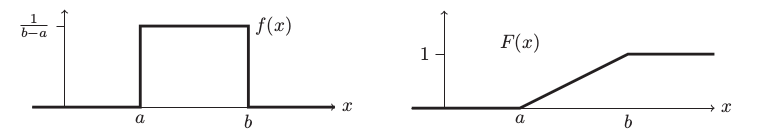
\includegraphics[scale=.35]{R1.png}
\end{figure}		
}
\end{frame}

\begin{frame}{Ejemplos}
\small{
\begin{enumerate}
\item Supongamos que tenemos una cinta m\'etrica con marcas en cada mil\'imetro. Si se mide  la longitud de los elementos que miden aproximadamente un metro de longitud, el error de redondeo se distribuir\'a uniformemente entre $-0.5$ y $0.5$ mil\'imetros.

\item Muchos juegos de mesa utilizan flechas giratorias (spinners) para introducir aleatoriedad. Cuando se hace girar, la flecha se detiene en un \'angulo que est\'a uniformemente distribuido entre $0$ y $2\pi$ radianes.

\item En la mayor\'ia de los generadores de n\'umeros pseudoaleatorios, el generador b\'asico simula una distribuci\'on uniforme y todas las dem\'as distribuciones se construyen mediante la transformaci\'on del generador b\'asico.
\end{enumerate}

\vspace{1.5cm}

}
\end{frame}

\begin{frame}{Distribuci\'on exponencial}
\small{
\begin{enumerate}
\item Param\'etros: $\lambda$.
\item Rango: $[a, \infty )$.
\item Notaci\'on: $\text{Exponencial}(\lambda)$.
\item Densidad: $f(x) = \lambda e^{-\lambda x}$ para $0\leq x$.
\item Distribuci\'on : $F(x) = 1 - e^{-\lambda x} \  \text{para}\  x \geq 0$ .
\item Distribuci\'on de la cola derecha: $\mathbb{P}(X > x) = 1 - F(x) = e^{-\lambda x}$.
\item Modelos: El tiempo de espera para un proceso continuo para cambiar el estado.	
\end{enumerate}

Gr\'aficos del PDF y el CDF de la distribuci\'on  $\text{Exponencial}(1)$:

\begin{figure}[ht]
	\centering
	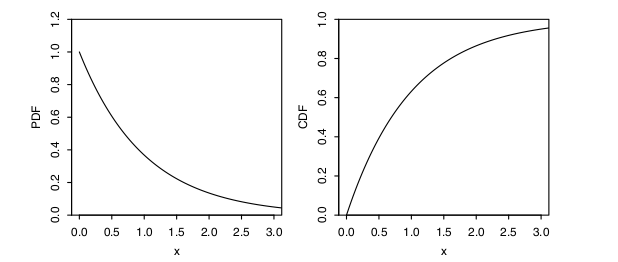
\includegraphics[height=2.5cm, width=8cm]{R2.png}
\end{figure}	
}
\end{frame}

\begin{frame}{Ejemplos}
\small{
\begin{enumerate}
\item Si salgo  77 Mass Ave después de  clases y espero el pr\'oximo taxi, mi tiempo de espera en minutos se distribuye exponencialmente. Veremos que en este caso $\lambda$ est\'a dado por uno sobre el promedio de taxis que pasan por minuto (en las tardes de los dias de semana).
\item La distribuci\'on exponencial modela el tiempo de espera hasta que un is\'otopo inestable sufra desintegraci\'on nuclear. En este caso, el valor de $\lambda $ est\'a relacionado con la semivida del is\'otopo.
\end{enumerate}

\vspace{2.5 cm}

}
\end{frame}

\begin{frame}{Memorylessness}
\small{Hay otras distribuciones que tambi\'en modelan los tiempos de espera, pero la distribuci\'on exponencial tiene la propiedad adicional de que no tiene memoria. En el contexto del primer ejemplo, supongamos que la probabilidad de que un taxi llegue dentro de los primeros cinco minutos es $p$. Si espero cinco minutos y de hecho no llega ning\'un taxi, entonces la probabilidad de que un taxi llegue dentro de los pr\'oximos cinco minutos sigue siendo $p$.
	

Formalmente, \textcolor{red}{\textbf{memoryless}} significa que la probabilidad de esperar $t$ m\'as minutos no se ve afectada por haber esperado $s$ minutos sin incidentes.

\vspace{0.2cm}

En s\'imbolos, $\mathbb{P}(X > s +t| X > s) = \mathbb{P}(X > t)$.

\vspace{0.2cm}


En efecto, desde que $(X >  s + t) \cap (X > s) = (X > s+ t)$, tenemos

\[
\mathbb{P}(X > s +t| X > s) = \frac{\mathbb{P}(X > s +t) }{\mathbb{P}(X > s) } = \frac{e^{-\lambda(s + t)}}{e^{-\lambda s}} = e^{-\lambda t} = \mathbb{P}(X > t).
\]

}
\end{frame}

\begin{frame}{Memorylessness}
\small{Por el contrario, supongamos que vamos a la estaci\'on de metro Miraflores y esperamos  al tren entrante. Dado que los trenes est\'an coordinados para seguir un horario (por ejemplo, aproximadamente $12$ minutos entre  trenes), si esperamos cinco minutos sin ver un tren, entonces hay una probabilidad mucho mayor de que un tren llegar\'a en los pr\'oximos cinco minutos.
	
En particular, el tiempo de espera para el metro no es sin memoria y un mejor modelo modelo  ser\'ia la distribuci\'on uniforme en el rango $[0,12]$.

\vspace{2.5cm}

}
\end{frame}

\begin{frame}{Distribuci\'on normal}
\small{
\begin{enumerate}
\item Param\'etros: $\mu, \sigma $.
\item Rango: $(-\infty, \infty )$.
\item Notaci\'on: $N(\mu, \sigma)$.
\item Densidad: $f(x) = \frac{1}{\sigma\sqrt{2\pi}} e^{-(x - \mu)^2/2\sigma^2}$ .
\item Distribuci\'on : $F(x)$ no tiene f\'ormula, as\'i usamos tablas o funciones como \textcolor{yellow}{\textbf{pnorm}} en R, para calcular $F(x)$.
\item Modelos: Error de medici\'on, inteligencia,habilidad, altura, promedios de muchos datos..
\end{enumerate}

Gr\'aficos del PDF y el CDF de la distribuci\'on  normal est\'andar $N(0,1)$:

\begin{figure}[ht]
\centering
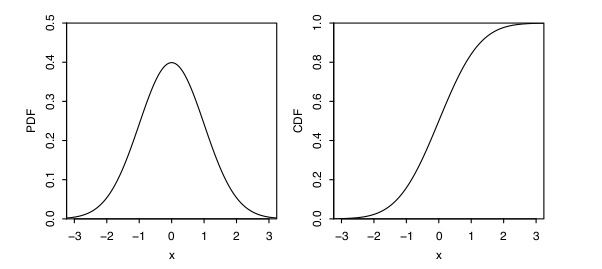
\includegraphics[height=2.5cm, width=8cm]{R3.png}
\end{figure}
}
\end{frame}

\begin{frame}{Distribuci\'on normal est\'andar}
\small{
	
La \textcolor{violet}{\textbf{distribuci\'on normal est\'andar}} $N(0,1)$ tiene media $0$ y varianza $1$. Reservamos $Z$ para la variable aleatoria est\'andar, $\varphi(z) = \frac{1}{\sqrt{2\pi}}e^{-x^2/2}$ para la densidad normal est\'andar y $\Phi(z)$ para la distribuci\'on normal est\'andar.

Hay varias propiedades de simetr\'ia importantes que se pueden deducir del PDF y CDF de la distribuci\'on normal est\'andar.

\begin{enumerate}
\item Simetr\'ia del PDF: $\varphi $ es una funci\'on  par.
\item Simetr\'ia de \'areas de cola:

El \'area bajo la curva del PDF a la izquierda de $-2$, que es  $P(Z \leq 2) = \Phi(-2)$ por definici\'on, es igual al \'area a la derecha de $2$, que es $\mathbb{P}(Z \geq  2) = 1 -\Phi(2)$. En general, tenemos

\[
\Phi(z) =  1 -\Phi(-z)
\]

\item Simetr\'ia de $Z$ y $-Z$: Si $Z \sim N(0,1)$ entonces $-Z \sim N(0,1)$.
\end{enumerate}
}
\end{frame}

\begin{frame}{Probabilidades normales}
\small{
Para hacer aproximaciones es \'util recordar la siguiente regla emp\'irica para tres probabilidades aproximadas

\[
\mathbb{P}(-1 \leq Z \leq 1) \approx 0.68, \ \mathbb{P}(-2 \leq Z \leq 2) \approx 0.95,\ \mathbb{P}(-3 \leq Z \leq 3) \approx 0.99,
\]

\begin{figure}[ht]
	\centering
	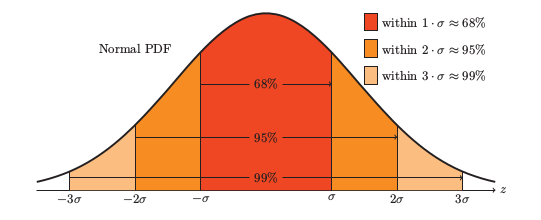
\includegraphics[height=2.5cm, width=8cm]{R4.png}
\end{figure}


Podemos usar la simetr\'ia de la distribuci\'on normal est\'andar alrededor de $x = 0$ para hacer algunos c\'alculos.
}
\end{frame}


\begin{frame}{Ejemplos}
\small{ Calculemos $\Phi(1)$,

\vspace{0.3cm}

	
Usando el resultado,$\mathbb{P}(-1 \leq Z \leq 1) \approx 0.68$,  $\Phi(1) = \mathbb{P}(Z \leq 1)$. 

En la figura, las dos colas (en rojo) han combinado el \'area $1 -0.68 = 0.32$. Por simetr\'ia la cola izquierda tiene \'area $0.16$ (la mitad de $0.32$), as\'i que $\mathbb{P}(Z \leq  1) \approx 0.68 + 0.16 = 0.84$.


\begin{figure}[ht]
	\centering
	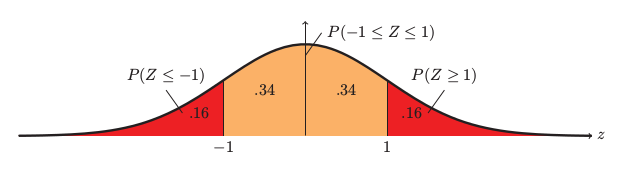
\includegraphics[height=2.5cm, width=8cm]{R5.png}
\end{figure}
}

\vspace{1.2cm}



\end{frame}

\begin{frame}{Distribuci\'on de Pareto}
\small{ 
\begin{enumerate}
\item Param\'etros: $m > 0 $ y  $\alpha > 0$.
\item Rango: $[m, \infty )$.
\item Notaci\'on: $\text{Pareto}(m, \alpha)$.
\item Densidad: $f(x) = \frac{\alpha m^{\alpha}}{x^{\alpha + 1}}$ .
\item Distribuci\'on : 
	
	\[
	F(x) = 1 - \frac{m^\alpha}{x^\alpha},\ \text{para}\ x \geq m.
	\]
	
\item Distribuci\'on  de la cola: $\mathbb{P}(X > x) = m^{\alpha}/x^{\alpha}$, para  $x \geq \alpha$.
\item Modelos: La distribuci\'on de Pareto modela una ley de potencia, donde la probabilidad de que ocurra un evento var\'ia como una potencia de alg\'un atributo del evento.

Muchos fen\'omenos siguen una ley de potencia, como el tama\~no de los meteoros, los niveles de ingresos en una poblaci\'on y los niveles de poblaci\'on en las ciudades.
\end{enumerate}

}
\end{frame}
\end{document}